\chapter{Variables, Expresiones y Sentencias}

Una de las más poderosas características de un lenguaje de programación
es la habilidad para manipular {\bf variables}. En términos generales, 
una variable es el nombre que hace referencia a un valor. Podría ser 
más preciso decir que una variable es un contenedor  
que tiene un nombre y que almacena un valor.
\index{variable}


\section{Sentencias de Asignación}
\label{variables}
\index{assignment!statement}
\index{statement!assignment}
\index{$=$ assignment operator}
\index{operator!assignment}


Una {\bf sentencia de asignación} usa el signo de igualdad {\tt =}
y le da un valor a una variable, pero, antes de que asignes un valor 
a una variable, debes primero crear la variable a través de una
declaración (si todavía no existe):
\begin{verbatim}
> my $mensaje;          # declración de una variable, aún sin valor
> $mensaje = 'And now for something completely different';
And now for something completely different
> my $número = 42;      # declaracion de una variable y asignación
42
> $número = 17;         # nueva asignación
17
> my $phi = 1.618033988;
1.618033988
>
\end{verbatim}
%
\index{assignment}
\index{statement!assignment}
\index{declaration!variable}
\index{variable!declaration}

Este ejemplos hace cuatros asignaciones. La primera asigna una cadena de texto
a una nueva variable llamada {\tt \$mensaje}, la segunda asigna 
el número entero {\tt 42} a {\tt \$número}, el tercero reasigna el entero {\tt 17} a
{\tt \$número}, y el cuarto asigna el valor aproximado del número áureo a {\tt \$phi}.

Aquí hay dos características sintácticas importantes que debes entender.

Primero, en Perl, los nombres de las variables comienzan un 
símbolo conocido como un {\emph sigilo}, i.e., un carácter no alfanumérico
como \verb'$', \verb'@', \verb'%', \verb'&', y otros más. Este carácter
especial nos dice y al compilador de Perl (el programa que lee
el código de nuestro programa y lo transfoma en instrucciones 
de computadoras) el tipo de variable que es. Por ejemplo, el 
carácter \$ indica que las variables más arriba son todas variables
escalares, lo cual significa que ellas pueden almacenar un solo valor
en cualquier momento. Veremos más adelante otros tipos de variables las
cuales pueden contener más de un solo valor.
\index{sigil}
\index{scalar}
\index{variable!scalar}
\index{scalar}

Segundo, nota como las tres variables más arriba son 
introducidas con la palabra clave {\tt my}, que es una manera
de declarar una variable nueva. Cuando tu creas una variable nueva
en Perl, necesitas \emph{declararla}, i.e., le deja saber a Perl
que vas a usar una variable nueva; esto se hace comúnmente con la
palabra clave {\tt my}, la cual declara una variable \emph{lexical}.
Explicaremos luego lo que es una variable lexical pero por ahora,
digamos que te permite crear una variable local a una parte 
limitada de tu código. Una de las buenas consecuencias del requerimiento
de declarar variables antes de que las uses es que, si tu cometes
un error al escribir el nombre de una variable, el compilador 
usualmente será capaz de decirte que estás usando una variable que
no ha sido declarada y como resultado te ayudará a encontrar tu error. 
Esto tiene grandes complicaciones las cuales examinaremos más tarde.
\index{my}
\index{declaring variables}
\index{variable!declaration}
\index{lexical}
\index{variable!lexical}

Cuando escribimos al inicio de esta sección que una variable debe
ser declarada antes de ser usada (o solo cuando se usa), esto
significa que la declaración tiene que ser antes (o al punto de) 
del primer uso de la variable en el archivo de texto que contiene el 
programa. Veremos más adelante que los programas no son ejecutados
necesariamente de arriba hacia abajo en el orden en el que las líneas
o código aparecen en el programa; aún así, la declaración de la variable
debe ser antes de su uso en el archivo de texto que contiene el programa.

Si olvidas declara una variable, obtienes un erro sintáctico:
\index{syntax error}

\begin{verbatim}
> $número = 5;
===SORRY!=== Error while compiling <unknown file>
Variable '$número' is not declared
at <unknown file>:1
------> <BOL><HERE>$número = 5;
>
\end{verbatim}
%
Ten presente que podrías obtener diferentes mensajes de
error dependiendo de la versión de Rakudo que ejecutes.
El mensaje arriba se obtuvo en Febrero 2016;
con una versión más nueva (Octubre 2016), el mismo error
se muestra en una forma algo más organizada:
\begin{verbatim}
>
> $número = 5;
===SORRY!=== Error while compiling:
Variable '$número' is not declared
at line 2
------> <BOL><HERE>$número = 5;
>
\end{verbatim}

\index{state diagram}
\index{diagram!state}

Una manera común de representar variables en papel es escribir el 
nombre con una flecha apuntando a su valor. Este tipo de dibujo se le conoce
como un {\bf diagrama de estado} porque muestra en qué estado cada una de las variables
se encuentra (imagínalo como el estado mental de la variable).
La figura\ref{fig.state2} muestra el resultado del ejemplo anterior.

\begin{figure}
\centerline
{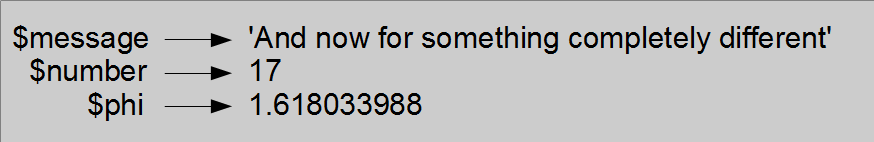
\includegraphics[scale=0.6]{figs/test_5.png}}
\caption{Diagrama de estado.}
\label{fig.state2}
\end{figure}



\section{Nombres de las Variables}
\index{variable}

Los programadores generalmente eligen nombres significativos
para sus variables---ellos documentan el uso de la variable.

Los nombres de las variables pueden ser tan largos como tu desees.
Ellos pueden contener letras y números, pero las variables
definidas por el usuario no pueden comenzar con un número. Los nombres de las
variables son sensibles al uso de mayúsculas y minúsculas, 
i.e., {\tt \$mensaje} no es la misma variable que {\tt \$Mensaje} 
o {\tt \$MENSAJE}. Es legal usar letras mayúsculas, pero es convencional
usar solo letras minúsculas para la mayoría de los nombres de las
variables. No obstante, algunas personas prefieren usar {\tt \$TipoTítulo}
para los nombres de sus variables o hasta {\tt \$MAYÚSCULAS} 
para algunas variables especiales.
\index{lower case}
\index{upper case}
\index{title case}
\index{case!lower}
\index{case!upper}
\index{case!title}


\index{Unicode}
\index{ASCII}
A diferencia de muchos otros lenguajes de programación, Perl~6 
no requiere que las letras y dígitos en los nombres de las variables
sean únicamente ASCII. Puedes usar cualquier tipo de letras Unicode, i.e.
letras de cualquier otro lenguaje en el mundo, así que, por ejemplo,
{\tt \$brücke}, {\tt \$payé} or {\tt \$niño} son nombres de variables
válidos, los cuales pueden ser usados por programadores que hablan 
otros idiomas diferentes al inglés (siempre y cuando estos caracteres
Unicode sean correctamente manipulados por tu editor de texto y tu
configuración de pantalla). De la misma manera, en vez de usar 
\verb"$phi" para el nombre de la variable del número aúreo,
podríamos haber usado la \emph{letra griega minúscula phi},
\verb'φ' (Unicode code point U+03C6). Igualmente, podríamos
haber usado la \emph{letra griega minúscula pi}, $\pi$, 
para la muy conocida razoń de la circunferencia del círculo
al diámetro:
\index{golden ratio}
\index{Unicode}
\index{phi}
\index{pi}

\begin{verbatim}
> my $φ = (5 ** .5 + 1)/2;       # número aúreo
1.61803398874989
> say 'Variable $φ = ', $φ;
Variable $φ = 1.61803398874989
> my $π = 4 * atan 1; 
3.14159265358979
> # podrías también las constante integrada pi o π:
> say pi
3.14159265358979
\end{verbatim}

El carácter de barra baja, \verb"_", puede aparecer en cualquier
parte del nombre de una variable. Usualmente se usa en nombres con
múltiples palabras, tal como \verb"$tu_nombre" o \verb"$airspeed_of_unladen_swallow". 
\index{underscore character}

Hasta puedes usar guiones para crear lo que se conoce como
``kebab case''\footnote{Porque las variables aparecen estar
atravesadas como las piezas de comida preparadas para un barbacoa.}
y nombrar esas variables \verb"$tu-nombre" or \verb"$airspeed-of-unladen-swallow",
y esto las puede hacer más legibles: un guión \verb'-' es válido en una variable
siempre y cuando sea inmediatamente seguido por un carácter alfanumérico.
Por ejemplo, \verb"$doble-clic" or \verb"$la-niña" son nombres legítimos
de variables. Análogamente, puedes usar un apóstrofo \verb"'" 
(también conocido como comilla simple) entre las letras, así que 
\verb"$isn't" o \verb"$o'brien's-age" son identificadores válidos. 
\index{dash}
\index{apostrophe}
\index{single quote}
\index{quote!single}
\index{kebab case}
\index{case!kebab}


Si les da un nombre ilegal a una variable, consigues 
un error sintáctico:
\index{syntax error}

\begin{verbatim}
> my $76trombones = 'big parade'
===SORRY!=== Error while compiling <unknown file>
Cannot declare a numeric variable
at <unknown file>:1
------> my $76<HERE>trombones = "big parade";
>
> my $more§ = 100000;
===SORRY!=== Error while compiling <unknown file>
Bogus postfix
at <unknown file>:1
------> my $more<HERE>§ = 100000;
(...)
\end{verbatim}
%
{\tt \$76trombones} es ilegal porque comienza con un número.
{\tt \$more§} es ilegal porque contiene un carácter ilegal, {\tt
§}. 

Si alguna vez has usado otro lenguaje de programación y 
te has tropezado con un mensaje terso tal como {\tt"SyntaxError: invalid syntax"},
notarás que los diseñadores de Perl han hecho un gran esfuerzo
para proveerte con mensajes de error que sean detallados, útiles
y significativos.
\index{error message}

Muchos lenguajes de programación tienen \emph{palabras claves} o
\emph{palabras reservadas} que son parte de la sintaxis, tales como
{\tt if}, {\tt while}, o {\tt for}, y por lo tanto no pueden ser usadas
para identificar variables porque eso crearía ambigüedad. Dicho problema
no existe en Perl: dado que los nombres de las variables comienzan un sigilo,
el compilador es siempre capaz de diferenciar entre una palabra clave
y una variable. Nombres tales como {\tt \$if} o {\tt \$while} son
sintácticamente identificadores válidos de variables en Perl 
(si estos nombres hacen sentido es un asunto diferente).
\index{sigil}
\index{keyword}
\index{reserved word}


\section{Expressions and Statements}
\label{expr_and_statements}

An {\bf expression} is a combination of terms and operators.
Terms may be variables or literals, i.e., constant values such as a number or a string. A value all by itself is considered an expression, and so is
a variable, so the following are all legal expressions:
\index{expression}
\index{term}
\index{literal}

\begin{verbatim}
> 42
42
> my $n = 17;
17
> $n;
17
> $n + 25;
42
>
\end{verbatim}
%
When you type an expression at the prompt, the interpreter
{\bf evaluates} it, which means that it finds the value of
the expression.
In this example, {\tt \$n} has the value 17 and
{\tt \$n + 25} has the value 42.
\index{evaluate}

A {\bf statement} is a unit of code that has an effect, like
creating a variable or displaying a value, and usually needs to end 
with a semi-colon {\tt ;} (but the semi-colon can sometimes be omitted 
as we will see later):
\index{statement}
\index{semi-colon}

\begin{verbatim}
> my $n = 17;
17
> say $n;
17
\end{verbatim}
%

The first line is an assignment statement that gives a value to
{\tt \$n}.  The second line is a print statement that displays the
value of {\tt \$n}.

When you type a statement and then press {\tt Enter}, the 
interpreter {\bf executes} it, which means that it does 
whatever the statement says.
\index{execute}

An assignment can be combined with expressions using arithmetic 
operators. For example, you might write:
\index{operator}

\begin{verbatim}
> my $answer = 17 + 25;
42
> say $answer;
42
\end{verbatim}
%

The \verb'+' symbol is obviously the addition operator 
and, after the assignment statement, the \verb'$answer' 
variable contains the result 
of the addition. The terms on each side of the operator 
(here 17 and 25) are sometimes called the \emph{operands} 
of the operation (an addition in this case).
\index{operand}
\index{addition operator}
\index{assignment}

Note that the REPL actually displays the result of the 
assignment (the first line with ``42''), so that the 
print statement was not really necessary in this 
example \emph{under the REPL}; from now on, for the sake of 
brevity, we will generally omit the print statements in the 
examples where the REPL displays the result.
\index{REPL}

In some cases, you want to add something to a variable 
and assign the result to that same variable. This could 
be written:

\begin{verbatim}
> my $answer = 17;
17
> $answer = $answer + 25;
42
\end{verbatim}
%

Here, \verb"$answer" is first declared with a value of 17. The next 
statement assigns to \verb"$answer" the current value of 
\verb"$answer" (i.e., 17) + 25. This is such a common operation 
that Perl, like many other programming languages, has a 
shortcut for this:

\begin{verbatim}
> my $answer = 17;
17
> $answer += 25;
42
\end{verbatim}
%

\index{$+=$ augmented assignment operator}
The \verb"+=" operator combines the arithmetic addition operator 
and the assignment operator to modify a value and apply the result 
to a variable in one go, so that \verb"$n += 2" means: take 
the current value of \verb"$n", add 2, and assign the result to 
\verb"$n". This syntax works with all other arithmetic operators. 
For example, \verb"-=" similarly performs a subtraction and an 
assignment, \verb"*=" a multiplication and an assignment, etc. It 
can even be used with operators other than arithmetic operators, 
such as the string concatenation operator that we will see later.

Adding 1 to a variable is a very common version of this, so that 
there is a shortcut to the shortcut, the \emph{increment} operator, 
which increments its argument by one, and returns the incremented value:
\index{increment operator}
\index{++ increment operator}
\index{operator!++ (increment)}

\begin{verbatim}
> my $n = 17;
17
> ++$n;
18
> say $n;
18
\end{verbatim}
%
This is called the prefix increment operator, because the \verb"++" 
operator is placed before the variable to be incremented. There is 
also a postfix version, \verb"$n++", which first returns the current 
value and then increments the variable by one. It would not make 
a difference in the code snippet above, but the result can be very different 
in slightly more complex expressions. 

There is also a decrement operator \verb"--", which decrements its 
argument by one and also exists in a prefix and a postfix form. 
\index{decrement operator}
\index{\verb'--' decrement operator}
\index{operator!$--$ (decrement)}



\section{Script Mode}

So far we have run Perl in {\bf interactive mode}, which
means that you interact directly with the interpreter (the 
REPL). Interactive mode is a good way to get started,
but if you are working with more than a few lines of code, 
it can be clumsy and even tedious.
\index{interactive mode}

The alternative is to use a text editor and save code in a file 
called a {\bf script} and then run the interpreter in {\bf script mode} 
to execute the script.  By convention, Perl~6 scripts have names that 
end with {\tt .pl}, {\tt .p6} or {\tt .pl6}.
\index{script}
\index{script mode}

Please make sure that you're really using a \emph{text editor} 
and not a \emph{word-processing program} (such as MS Word, 
OpenOffice or LibreOffice Writer). There is a very large 
number of text editors available for free. On Linux, you might use 
\emph{vi} (or \emph{vim}), \emph{emacs}, \emph{gEdit}, or 
\emph{nano}. On Windows, you may use \emph{notepad} (very limited) 
or \emph{notepad++}. There are also many cross-platform editors  
or integrated development environments (IDEs) providing a 
text editor functionality, including \emph{padre}, \emph{eclipse}, 
or \emph{atom}. Many of these provide various syntax highlighting 
capabilities, which might help you use correct syntax (and 
find some syntax errors).
\index{syntax!highlighting}
\index{text editor!emacs}
\index{text editor!vi}
\index{text editor!vim}
\index{text editor!gEdit}
\index{text editor!padre}
\index{text editor!eclipse}
\index{text editor!nano}
\index{text editor!notepad++}
\index{text editor!atom}

Once you've saved your code into a file (say, for example, 
\verb'my_script.pl6'), you can run the program by issuing 
the following command at the operating system prompt (for example 
in a Linux console or in a \verb'cmd' window under Windows):
\begin{verbatim}
perl6 my_script.pl6
\end{verbatim}

Because Perl provides both modes,
you can test bits of code in interactive mode before you put them
in a script.  But there are differences between interactive mode
and script mode that can be confusing.
\index{interactive mode}
\index{script mode}

For example, if you are using the Perl~6 interpreter as a 
calculator, you might type:

\begin{verbatim}
> my $miles = 26.2;
26.2
> $miles * 1.61;
42.182
\end{verbatim}

The first line assigns a value to {\tt \$miles} and displays that value.  
The second line is an expression, so the
interpreter evaluates it and displays the result.  It turns out that a
marathon is about 42~kilometers.

But if you type the same code into a script and run it, you get no
output at all.  In script mode, an expression, all by itself, has no
visible effect.  Perl actually evaluates the expression, but it doesn't
display the value unless you tell it to:

\begin{verbatim}
my $miles = 26.2;
say $miles * 1.61;
\end{verbatim}

This behavior can be confusing at first. Let's examine why.

A script usually contains a sequence of statements.  If there
is more than one statement, the results appear one at a time
as the print statements execute.

For example, consider the following script:

\begin{verbatim}
say 1;
my $x = 2;
say $x;
\end{verbatim}
%
It produces the following output:

\begin{verbatim}
1
2
\end{verbatim}
%
The assignment statement produces no output.

To check your understanding, type the following statements in the
Perl interpreter and see what they do:

\begin{verbatim}
5;
my $x = 5;
$x + 1;
\end{verbatim}

Now put the same statements in a script and run it.  What
is the output?  Modify the script by transforming each
expression into a print statement and then run it again.

\section{One-Liner Mode}

Perl also has a \emph{one-liner mode}, which enables you 
to type directly a very short script at the operating 
system prompt. Under Windows, it might look like this:
\index{one-liner mode}
\label{one-liner mode}

\begin{verbatim}
C:\Users\Laurent>perl6 -e "my $value = 42; say 'The answer is ', $value;"
The answer is 42

\end{verbatim}

The {\tt -e} option tells the compiler that the script to 
be run is not saved in a file but instead typed at the 
prompt between quotation marks immediately after 
this option.

Under Unix and Linux, you would replace double quotation 
marks with apostrophes (or single quotes) 
and apostrophes with double quotation marks:
\index{apostrophe}
\index{quote mark}

\begin{verbatim}
$  perl6 -e 'my $value = 42; say "The answer is $value";'
The answer is 42

\end{verbatim}

The one-liner above may not seem to be very useful, but 
throwaway one-liners can be very practical to perform 
simple one-off operations, such as quickly modifying 
a file not properly formatted, without having to save a script 
in a separate file before running it.

We will not give any additional details about the one-liner 
mode here, but will give some more useful examples 
later in this book; for example, 
Subsection~\ref{one-liner-example},
Subsection~\ref{rot13_oneliner} (solving the ``rot-13'' exercise), or
Subsection~\ref{sol_cartalk} (solving the exercise on 
consecutive double letters). 



\section{Order of Operations}
\index{order of operations}
\index{PEMDAS}
\index{operator precedence}
\index{precedence!operator}

When an expression contains more than one operator, the order of
evaluation depends on the {\bf order of operations} or \emph{operator precedence}. 
For mathematical operators, Perl follows mathematical convention.
The acronym {\bf PEMDAS}\footnote{US students are sometimes taught 
to use the "Please Excuse My Dear Aunt Sally" mnemonics to remember 
the right order of the letters in the acronym.} is a useful 
way to remember the rules:

\begin{itemize}

\item {\bf P}arentheses have the highest (or tightest) precedence and can be used 
to force an expression to evaluate in the order you want. Since
expressions in parentheses are evaluated first, {\tt 2 * (3-1)} is 4,
and {\tt (1+1)**(5-2)} is 8. You can also use parentheses to make an
expression easier to read, as in {\tt (\$minute * 100) / 60}, even
if it doesn't change the result.
\index{$()$ parenthesis operator}

\item {\bf E}xponentiation has the next highest precedence, so
{\tt 1 + 2**3} is 9 (1 + 8), not 27, and {\tt 2 * 3**2} is 18, not 36.
\index{$**$ exponentiation operator}
\index{operator!$**$ (exponentiation)}

\item {\bf M}ultiplication and {\bf D}ivision have higher precedence
  than {\bf A}ddition and {\bf S}ubtraction.  So {\tt 2*3-1} is 5, not
  4, and {\tt 6+4/2} is 8, not 5.
\index{$*$ multiplication operator}
\index{operator!$*$ (multiplication)}
\index{$/$ division operator}
\index{operator!$/$ (division)}

\item Operators with the same precedence are usually evaluated 
from left to right (except exponentiation).  So in the expression 
{\tt \$degrees / 2 * pi}, the division happens first and the 
result is multiplied by {\tt pi}, which is not the expected 
result. (Note that {\tt pi} is not a variable, but a predefined 
constant in Perl~6, and therefore does not require a sigil.)  To 
divide by $2 \pi$, you can use parentheses:
\index{sigil}
\index{pi}
  
\begin{verbatim}
my $result = $degrees / (2 * pi);  
\end{verbatim}  
 
or write
  {\tt \$degrees / 2 / pi} or {\tt \$degrees / 2 / $\pi$}, which
  will divide \verb'$degrees' by 2, and then divide the result of 
  that operation by $\pi$ (which is equivalent to \verb'$degrees'
  divided by $2 \pi$).

\end{itemize}

I don't work very hard to remember the precedence of
operators.  If I can't tell by looking at the expression, I use
parentheses to make it obvious. If I don't know for sure which of two operators 
has the higher precedence, then the next person reading or maintaining 
my code may also not know.
\index{precedence}
\index{parentheses}


\section{String Operations}
\label{string_operations}
\index{string!operation}
\index{operator!string}
\index{coercion}
\index{type!coercion}

In general, you can't perform mathematical operations on strings, unless
the strings look so much like numbers that Perl can transform or \emph{coerce} them into numbers and still make sense, so the 
following are illegal:

\begin{verbatim}
'2'-'1a'    'eggs'/'easy'    'third'*'a charm'
\end{verbatim}
%

For example, this produces an error:

\begin{verbatim}
> '2'-'1a'
Cannot convert string to number: trailing characters after number 
in '1?a' (indicated by ?)
  in block <unit> at <unknown file>:1
\end{verbatim}
%
  
But the following expressions are valid because these strings 
can be coerced to numbers without any ambiguity:
\begin{verbatim}
> '2'-'1'
1
> '3'/'4'
0.75
\end{verbatim}
%

The \verb'~' operator performs {\bf string concatenation}, which means
it joins the strings by linking them end-to-end.  For example:
\index{string concatenation}
\index{string!concatenation}

\begin{verbatim}
> my $first = 'throat'
throat
> my $second = 'warbler'
warbler
> $first ~ $second
throatwarbler
\end{verbatim}
%
The {\tt x} operator also works on strings; it performs repetition.
For example:
\index{string repetition}

\begin{verbatim}
> 'ab' x 3;
ababab
> 42 x 3
424242
> 3 x 42
333333333333333333333333333333333333333333
\end{verbatim}

Notice that, although the {\tt x} operator somewhat looks like 
the multiplication operator when we write it by hand, {\tt x} 
is obviously not commutative, contrary to the {\tt *} 
multiplication operator. The first operator is a string or is 
\emph{coerced} to a string (i.e., transformed into a string: 
{\tt 42} is coerced to {\tt '42'}), and the second operator 
has to be a number or something that can be transformed 
into a number.
\index{commutativity}
\index{coercion}


\section{Comments}
\index{comment}

As programs get bigger and more complicated, they get more difficult
to read.  Formal languages are dense, and it is often difficult to
look at a piece of code and figure out what it is doing, or why.

For this reason, it is a good idea to add notes to your programs to explain
in natural language what the program is doing.  These notes are called
{\bf comments}, and they start with the \verb"#" symbol:

\begin{verbatim}
# compute the percentage of the hour that has elapsed
my $percentage = ($minute * 100) / 60;
\end{verbatim}
%
In this case, the comment appears on a line by itself.  You can also put
comments at the end of a line:

\begin{verbatim}
$percentage = ($minute * 100) / 60;     # percentage of an hour
\end{verbatim}
%
Everything from the {\tt \#} to the end of the line is ignored---it
has no effect on the execution of the program.

Comments are most useful when they document nonobvious features of
the code.  It is reasonable to assume that the reader can figure out
{\em what} the code does; it is more useful to explain {\em why}.

This comment is redundant with the code and useless:

\begin{verbatim}
my $value = 5;        # assign 5 to $value
\end{verbatim}
%
This comment, by contrast, contains useful information that 
is not in the code:

\begin{verbatim}
my $velocity = 5;     # velocity in meters/second. 
\end{verbatim}
%
Good variable names can reduce the need for comments, but
long names can make complex expressions hard to read, so there is
a tradeoff.
\index{variable name}


\section{Debugging}
\index{debugging}
\index{bug}

Three kinds of errors can occur in a program: syntax errors, runtime 
errors, and semantic errors.  It is useful
to distinguish between them in order to track them down more quickly.

\begin{description}

\item[Syntax error] ``Syntax'' refers to the structure of a program
  and the rules about that structure.  For example, parentheses have
  to come in matching pairs, so {\tt (1 + 2)} is legal, but 
{\tt 8)} is a \emph{syntax error}. \footnote{We are using 
``syntax error'' here as a quasi-synonym for ``compile-time error''; 
they are not exactly the same thing (you may in theory have 
syntax errors that are not compile-time errors and the other way 
around), but they can be deemed to be the same for 
practical purposes here. In Perl~6, compile-time errors 
have the ``===SORRY!==='' string at the beginning of 
the error message.}

\index{error!syntax}
\index{error message}
\index{syntax} 
\index{syntax!error}

If there is a syntax error
anywhere in your program, Perl displays an error message and quits 
without even starting to run your program, and you will 
obviously not be able to run the program.  During the first few
weeks of your programming career, you might spend a lot of
time tracking down syntax errors.  As you gain experience, you will
make fewer errors and find them faster.


\item[Runtime error] The second type of error is a runtime error, so
  called because the error does not appear until after the program has
  started running.  These errors are also called \emph{exceptions}
  because they usually indicate that something exceptional (and bad)
  has happened.  \index{runtime error} \index{error!runtime}
  \index{exception} \index{safe language} \index{language!safe}

Runtime errors are rare in the simple programs you will see in the
first few chapters, so it might be a while before you encounter one. 
We have seen one example of such errors, though, at the beginning 
of Section~\ref{string_operations} (p.~\pageref{string_operations}), 
when we tried to subtract \verb"'2'-'1a'". 


\item[Semantic error] The third type of error is \emph{semantic}, which
  means related to meaning.  If there is a semantic error in your
  program, it will run without generating error messages, but it will
  not do the right thing.  It will do something else.  Specifically,
  it will do what you \emph{told} it to do, but not what you 
  \emph{intended} it to do.
  \index{semantic error}
  \index{error!semantic} \index{error message}

Identifying semantic errors can be tricky because it requires you to work
backward by looking at the output of the program and trying to figure
out what it is doing.

\end{description}


\section{Glossary}

\begin{description}

\item[Variable]  Informally, a name that refers to a value. More 
accurately, a variable is a container that has a name and holds a value.
\index{variable}

\item[Assignment]  A statement that assigns a value to a variable.
\index{assignment}

\item[State diagram]  A graphical representation of a set of variables and the
values they refer to.
\index{state diagram}

\item[Keyword]  A reserved word that is used to parse a
program; in many languages, you cannot use keywords like 
{\tt if}, {\tt  for}, and {\tt while} as variable names. 
This problem usually does not occur in Perl because variable
names begin with a \emph{sigil}.
\index{keyword}
\index{sigil}

\item[Operand] A value or term next to an operator that 
is used in its evaluation.
\index{operand}

\item[Term]  A variable or a literal value.
\index{term}

\item[Expression]  A combination of operators and terms that
represents a single result.
\index{expression}

\item[Evaluate]  To simplify an expression by performing the operations
in order to yield a single value.
\index{evaluate}

\item[Statement]  A section of code that represents a command or action.  So
far, the statements we have seen are assignments and print statements. Statements usually end with a semi-colon.
\index{statement}

\item[Execute]  To run a statement and do what it says.
\index{execute}

\item[interactive mode (or interpreter mode):] A way of using the Perl 
interpreter by typing code at the prompt.
\index{interactive mode}

\item[Script mode] A way of using the Perl interpreter to read
code from a script and run it.
\index{script mode}

\item[one-liner mode:] A way of using the Perl interpreter to read
code passed at the operating system prompt and run it.
\index{one-liner mode}

\item[Script] A program stored in a file.
\index{script}

\item[Order of operations]  Rules governing the order in which
expressions involving multiple operators and operands are evaluated.
It is also called operator precedence.
\index{order of operations}
\index{operator precedence}
\index{precedence!operator}

\item[Concatenate]  To join two string operands end-to-end.
\index{concatenation}

\item[Comment]  Information in a program that is meant for other
programmers (or anyone reading the source code) and has no effect on the
execution of the program.
\index{comment}

\item[Syntax error]  An error in a program that makes it impossible
to parse (and therefore impossible to compile and to run).
\index{syntax!error}

\item[Exception]  An error that is detected while the program is running.
\index{exception}

\item[Semantics]  The meaning of a program.
\index{semantics}

\item[Semantic error]   An error in a program that makes it do something
other than what the programmer intended.
\index{semantic error}

\end{description}


\section{Exercises}

\begin{exercise}

Repeating our advice from the previous chapter, whenever you learn
a new feature, you should try it out in interactive mode (under 
the REPL) and make errors on purpose to see what goes wrong.
\index{interactive mode}
\index{REPL}

\begin{itemize}

\item We've seen that {\tt \$n = 42} is legal.  What about {\tt 42 = \$n}?

\item How about {\tt \$x = \$y = 1}? (Hint: note that you will 
have to declare both variables, for example with a statement 
such as {\tt my \$x; my \$y;} or possibly {\tt my (\$x, \$y);}, 
before you can run the above.)

\item In some languages, statements don't have to end with a semi-colon, 
{\tt ;}. What happens in script mode if you omit a semi-colon at the end
of a Perl statement?
\index{semi-colon}

\item What if you put a period at the end of a statement?

\item In math notation you can multiply $x$ and $y$ like this: $x y$.
What happens if you try that in Perl?

\end{itemize}

\end{exercise}


\begin{exercise}

Practice using the Perl interpreter as a calculator: 
\index{calculator}

\begin{enumerate}

\item The volume of a sphere with radius $r$ is $\frac{4}{3} \pi r^3$.
  What is the volume of a sphere with radius 5?

\item Suppose the cover price of a book is \$24.95, but bookstores get a
  40\% discount.  Shipping costs \$3 for the first copy and 75 cents
  for each additional copy.  What is the total wholesale cost for
  60 copies?

\item If I leave my house at 6:52 a.m. and run 1 mile at an easy pace
  (8:15 per mile), then 3 miles at tempo (7:12 per mile) and 1 mile at
  easy pace again, what time is it when I complete my running exercise?
\index{running pace}

\end{enumerate}
\end{exercise}

